% !TeX root = 00_main.tex

\chapter{Trajectory based user identification}
\label{sec:method}

Trajectory models are introduced to capture the motion of a user $u\in\mathcal{U}$ in space and time by learning from their trajectory profile $\mathcal{P}(u)$ in Subsection \ref{subsec:modeling}. For each model, a similarity measure to quantify similarity between different trajectory models is proposed. Based on these similarity measures, the user identification approach is presented in Subsection \ref{subsec:class}. As mentioned before, the prediction is based on the assumption that there exists a profile $P(u_i)$ for each user $u_i \in U$.

\section{Trajectory Profile Modeling}\label{subsec:modeling}
Each trajectory $\mathcal{\DB}(u, e)$ of user $u$ during epoch $e$ is a sequence of observations, i.e., time-stamped geo-locations. A spatial grid to partition geo-space into equal sized regions $\mathcal{S}=\{S_1,S_{|S|}\}$ is used, thus reducing a trajectory to a sequence of time-stamped grid-cells. To model such a sequence, two kinds of approaches are proposed:
\begin{itemize}
\item The first approach using \emph{set descriptors} treats a trajectory as a \emph{set} of grid-cell observations, thus ignoring the sequence, ordering, and time-stamps of these observations.
\item The second approach using \emph{frequent transitions} considers the transitions of users from one spatial region to another, thus explicitly modeling the order of observations.
\end{itemize}

\subsection{Set Descriptors}\label{subsubsec:set}
Ignoring the temporal aspect, a trajectory $\DB(u, e)$ of user $u$ during epoch $e$ can be described by a vector $v(u,e)$ all spatial regions in $S$. In other words, each spatial region is represented by a dimension of $v(u,e)$.

Note that $v(u,e)$ contains zero values in the majority of dimensions as each user usually only traverses a small fraction of space during an epoch. In other words, $v(u,e)$ is sparse.
Modeling trajectories using frequency descriptions has a strong resemblance to handling bag of words vectors known in text mining. To describe, if and how often a domain was visited within trajectory $\DB(u,e)$, the following two approaches are examined.

Simple examples of these can be seen in Figure \ref{fig:trajectory_creation}. Each color represents different users geotagging in the area of interest. Then a 4x4 grid is applied to the area, and set descriptors are generated from the data.

\begin{figure}[ph]
	\centering
	\begin{subfigure}[b]{\textwidth}
		\centering
		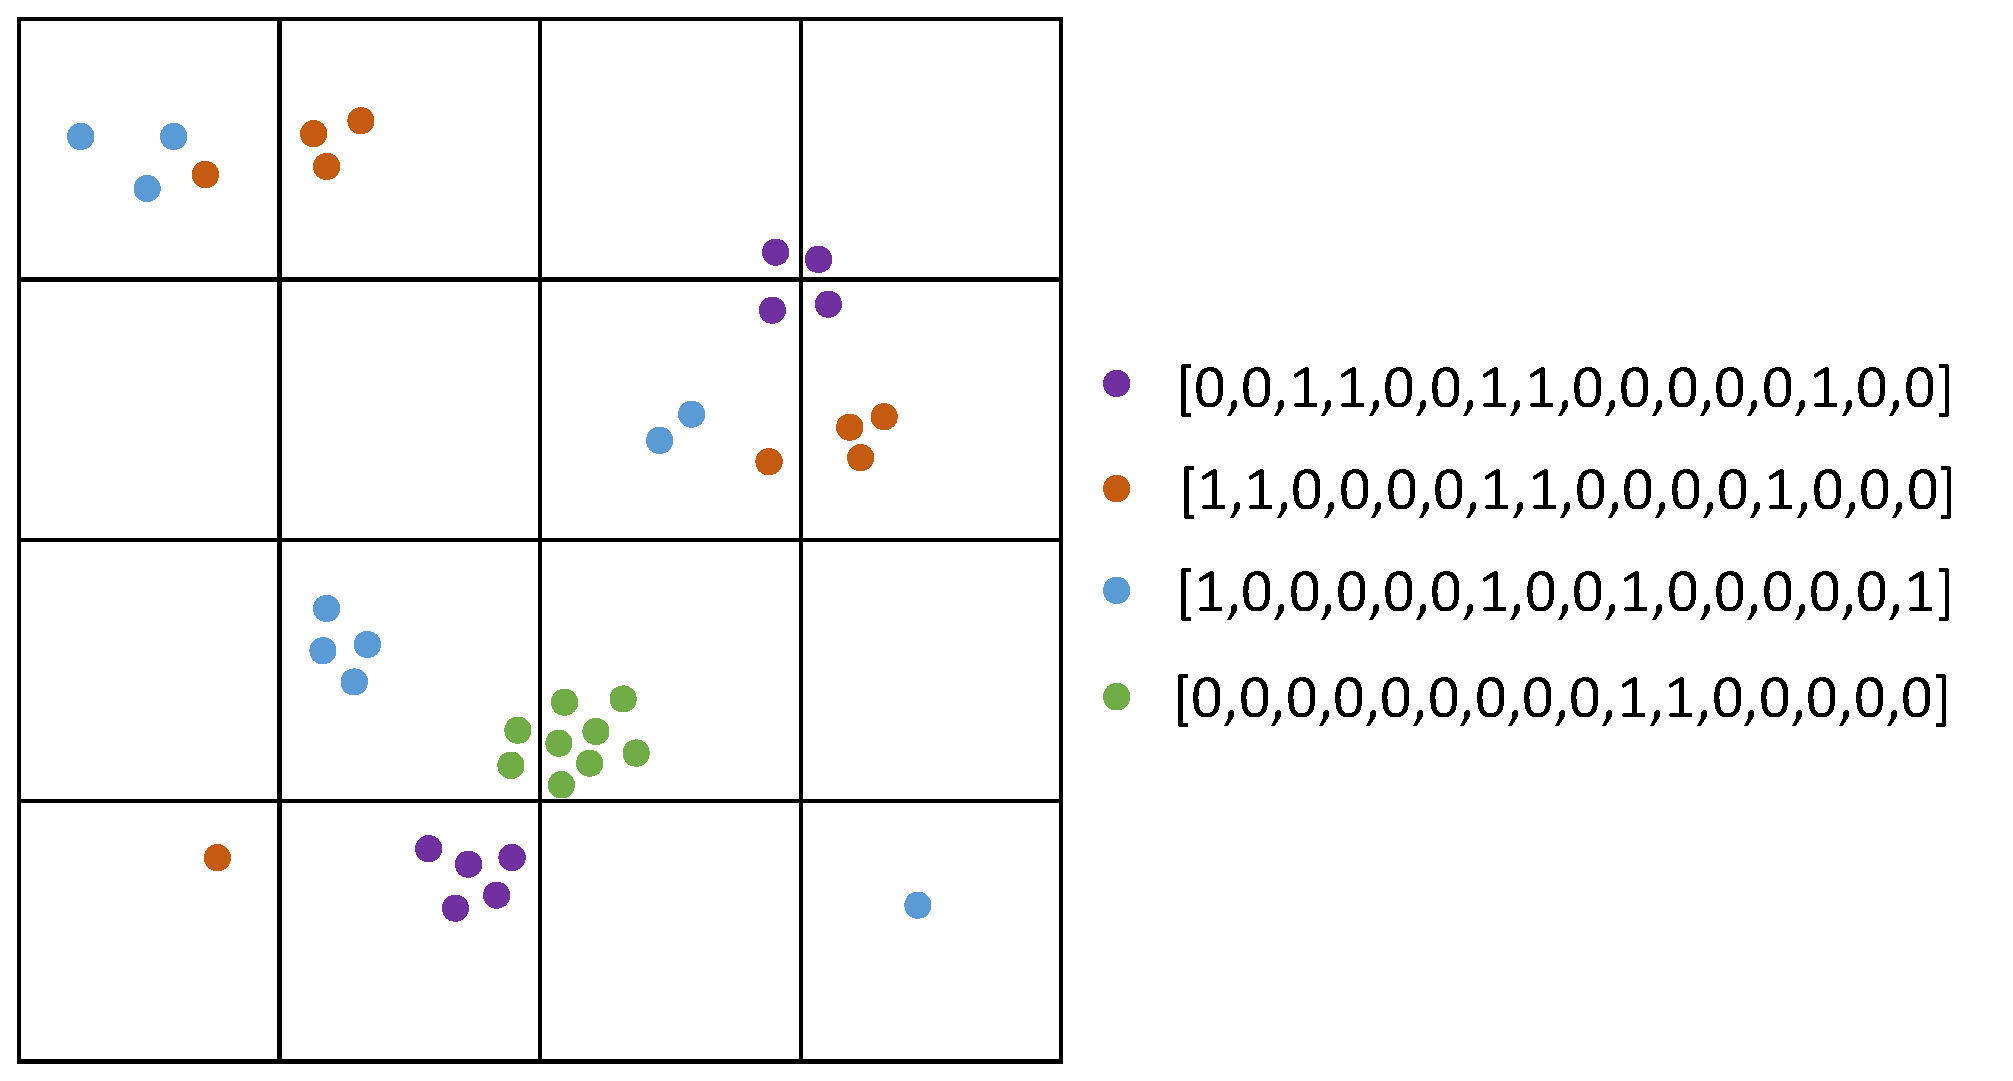
\includegraphics[width = 0.9\textwidth]{figures/trajectory_bitset}
		\subcaption{Bitset Descriptor}
    \label{fig:trajectory_bitset}
	\end{subfigure}

	\begin{subfigure}[b]{\textwidth}
		\centering
		\includegraphics[width = 0.9\textwidth]{figures/trajectory_frequency}
		\subcaption{Frequency Descriptor}
  	\label{fig:trajectory_frequency}
	\end{subfigure}
  \caption{Set descriptor trajectory creation.}
  \label{fig:trajectory_creation}
	\figSpace
\end{figure}

\paragraph{Bitset Descriptor}
In this rather simple method, a trajectory $\DB(u,e)$ is represented as a set of visited spatial regions. Thus, each feature value $v^{\mbox{bit}}$ equals one if user $u$ visited region $S_i$ (at least once) during epoch $e$, formally:
$$
v^{\mbox{bit}}_i (u,e):=
\begin{cases}
        1,& \text{if }\exists (u^\prime,s,t)\in\DB: u^\prime=u \wedge s\in S_i \wedge t\in e,\\
        0, & \text{otherwise}
        \end{cases}
$$
A visual example of this is shown in \ref{fig:trajectory_bitset}.

To compare bitset vectors $v, v^\prime  \in \{0,1\}^n$, the Jaccard coefficient is employed, which is a standard similarity measure for sets:
\begin{definition}[Jaccard Coefficient]
Let $v,v^\prime \in \{0,1\}^n$ be two bit vectors, then the Jaccard coefficient is defined as follows:
\begin{displaymath}
Jac(v,v^\prime)=\frac{\sum_{i=1}^n v_i \wedge v_i^\prime}{\sum_{i=1}^n v_i \vee v_i^\prime}
\end{displaymath}
\end{definition}

\paragraph{Frequency Descriptors}
A frequency vector $v^{\mbox{freq}}$ contains the number of visits of each spatial region of user $u$ in epoch $e$. This allows to distinguish between users visiting a particular region more or less often than other users.
$$
v^{\mbox{freq}}(u,e)_i=|\{(u^\prime,s,t)\in\DB|u^\prime=u \wedge s\in S_i \wedge t\in e\}|.
$$
A visual example of this is shown in \ref{fig:trajectory_frequency}.

The standard way to compute the similarity in sparse numerical vectors is the cosine coefficient:
\begin{definition}[Cosine Coefficient]
Let $v,v^\prime \in \NN^n$ be two vectors, then the Cosine coefficient is defined as follows:
\begin{displaymath}
Cos(v,v^\prime)=\frac{v^T \cdot v^\prime}{||v|| \cdot ||v^\prime||}
\end{displaymath}
\end{definition}
Since the cosine coefficient can be strongly dominated by dimensions having high average frequency values, spatial regions are normalized by their total number of observations.

\subsection{Transition Descriptors}\label{subsubsec:trans}
All of the previous trajectory descriptors had in common that they treat a trajectory as an unordered set of locations, without considering any notion of sequence or time. In this section, a trajectory is treaded as a sequence of regions. As a baseline to compute the similarity between two sequences, dynamic time-warping \cite{Berndt1994} (DTW), a state-of-the-art method for similarity search on sequences, is used. Since the experimental evaluation shows that using DTW without any adaption as a similarity measure yields a fairly low classification accuracy, this section presents two approaches to directly model the transitions of a trajectory. A transition is a pair $(s,s^\prime)$ of regions where $s$ is called source and $s^\prime$ is called destination. Using a descriptor for each pair of spatial regions $s_i,s_j$, describing the number of times the specific sequence $(s_i,s_j)$ has been observed in a trajectory $\DB(u,e)$, is proposed.

\begin{definition}[Trajectory Transitions]
Let $\DB(u,e)=\{(s_1,t_1),...,(s_n,t_n))\}$ be a trajectory, the set of transitions $\uparrow\DB(u,e)$ is defined as the multi-set (thus allowing duplicates)
$$
\uparrow\DB(u,e):=\bigvee_{1\leq i< n}(s_i,s_{i+1}).
$$
The number of occurrences of $(s,s^\prime)$ in trajectory $\DB(s,e)$ is denoted as $\uparrow\DB(u,e)(s,s^\prime)$.
\end{definition}
Since modeling all observed transitions blows up the feature space quadratically, Using only the $k$ globally most frequent transitions as features is proposed.
\begin{itemize}
  \item {\bf Frequent Transitions:} The globally most frequent transitions are searched for and the number of occurrences of these transitions is used as a feature vector to describe a trajectory.
  \item {\bf Transition Probabilities:} Common transitions of two trajectories are found, and their similarities are adapted by the global rarity of these transitions.
\end{itemize}

\begin{definition}[Top-$k$ Most Frequent Transitions]
Let $k$ be a positive integer, then the set $FT$ is a set of pairs of spatial regions defined as
$$
FT^k(\DB)=argmax^k_{s_i,s_j\in \mathcal{S}} |\{\sum_{u\in\mathcal{U},e\in\mathcal{E}}\uparrow\DB(u,e)(s_i,s_j)\}|,
$$
where $argmax^k_X(\varphi)$ returns the set of $k$ arguments $x\in y$ yielding the maximum value substituted in term $\varphi$.
\end{definition}
Now the $k$ most frequent transitions $FT^k(\DB)$ can be used as additional features.
Similar to the set descriptors presented in Subsection \ref{subsubsec:set}, the features are described using
\begin{itemize}
\item Bit vectors, using the feature vector
$$
v^{\uparrow\mbox{bit}(u,e)}_i=\begin{cases}1 & \text{if }FT^k(\DB)_i\in \uparrow\DB(u,e) \\ 0 & \text{otherwise}\end{cases}
$$
\item Frequency vectors, using the feature vector
$$
v^{\uparrow\mbox{freq}}(u,e)_i=\uparrow\DB(u,e)(FT^k(\DB)_i)
$$

\end{itemize}
For these vectors, the same similarity functions defined in Section \ref{subsubsec:set} can be used.

\section{Classification}\label{subsec:class}
Regardless of which of the modeling approaches presented in this section is employed, the result is a high-dimensional feature vector. To classify a new trajectory of an unknown user, the next section proposes the classification procedure, using the previously proposed user-specific trajectory models. To classify the user of a new trajectory, a $k$-nearest neighbor classification approach is employed. This choice is made due to the extremely high dimensional feature space, having one dimension per spatial grid-cell.
Therefore, given a trajectory database $\DB$, trajectories $\DB(u,e)$ are extracted for each user $u$ in each epoch $e$. Since the user is known for each of these trajectories, the result is a labeled dataset $P_{train}$ of feature vectors. Given a new trajectory $Q$, map $Q$ to its feature description $v_{new}$ and search the $k$-nearest neighbors of $v_{new}$ in $P_{train}$ w.r.t. a corresponding similarity measure. To decide the final class decision, each queried neighbor is weighted by its similarity value and the class is predicted as the one having the largest cumulated similarity.

Formally, this can be define the $k$-nearest neighbors classification as follows.
Let $P_{train} = \lbrace (v_i, y_i)~\vert~v_i \in \lbrace 0, 1\rbrace ^n \wedge y_i \in \mathcal{L} \rbrace$ be the set of training instances consisting of pairs $(v_i, y_i)$ with $v_i$ being the feature description of the user trajectory $i$ and $y_i$ being the label, i.e., identity of the user, assigned to trajectory $i$. $\mathcal{L}$ denotes the set of labels.
Given the feature description $v_{new}$ of a query trajectory, the identity, resp. label, $y_{new}$ of $v_{new}$ is determined by cumulating the similarities, i.e., $d(.,.)$, for each label $l \in \mathcal{L}$ represented among the $k$-nearest neighbors of $v_{new}$ and taking the most representative label.
$$y_{new} = argmax_{l \in \mathcal{L}} \lbrace \sum{d(v_{new}, v_k^l)}~\vert~v_k^l \in kNN(v_{new}) \rbrace$$
Note that no index structure is used to support the $k$NN-search due to the high dimensionality of the feature space.

\section{User Linkage}\label{subsec:linkage}
In addition to the identification of individual users, another application of the user trajectory profiling is to link users between two trajectory datasets. Therefore, let $\DB$ and $\DB^\prime$ be two trajectory databases having the set of users $\mathcal{U}$ and $\mathcal{U}^\prime$, respectively. The task of user linkage is to find pairs of database users $(u\in\mathcal{U},u^\prime\in\mathcal{U}^\prime)$ that correspond to the same individual in the real world, i.e., having $u=u^\prime$. As an example, the two data sets may correspond to Twitter and Instagram. The same individual may have different user names in both social networks. The task of user linkage is to find such individuals.

Clearly, using the approach presented in Section \ref{subsec:class}, the trajectories of each user are classified in $\DB$, and the most similar user in $\DB^\prime$ is classified. The drawback of such approach is that multiple users in $\DB$ may be matched to the same user in $\DB^\prime$, and some users in $\DB\prime$ might not have any match. To avoid this drawback, the matching problem is formalized as a bipartite graph, containing for each $(u\in\mathcal{U},u^\prime\in\mathcal{U}^\prime)$ a weight of similarity. This similarity is chosen by performing a $k$NN search of each trajectory in $\DB$ on the database $\DB^\prime$. Then, the score of $(u,u^\prime)$ corresponds to the number of occurrences of $u\prime$ in $k$NN sets of all trajectories of user $u$.

Given this bipartite graph, the Hopcroft-Karp algorithm \cite{Hopcroft1973} is used to find an optimal matching, i.e., mapping of each user in the smaller database to exactly one user in the other that maximizes the total score.
